%!TEX TS-program = xelatex

% Шаблон документа LaTeX создан в 2018 году
% Алексеем Подчезерцевым
% В качестве исходных использованы шаблоны
% 	Данилом Фёдоровых (danil@fedorovykh.ru) 
%		https://www.writelatex.com/coursera/latex/5.2.2
%	LaTeX-шаблон для русской кандидатской диссертации и её автореферата.
%		https://github.com/AndreyAkinshin/Russian-Phd-LaTeX-Dissertation-Template

\documentclass[a4paper,14pt]{article}


%%% Работа с русским языком
\usepackage[english,russian]{babel}   %% загружает пакет многоязыковой вёрстки
\usepackage{fontspec}      %% подготавливает загрузку шрифтов Open Type, True Type и др.
\defaultfontfeatures{Ligatures={TeX},Renderer=Basic}  %% свойства шрифтов по умолчанию
\setmainfont[Ligatures={TeX,Historic}]{Times New Roman} %% задаёт основной шрифт документа
\setsansfont{Comic Sans MS}                    %% задаёт шрифт без засечек
\setmonofont{Courier New}
\usepackage{indentfirst}
\frenchspacing

\renewcommand{\epsilon}{\ensuremath{\varepsilon}}
\renewcommand{\phi}{\ensuremath{\varphi}}
\renewcommand{\kappa}{\ensuremath{\varkappa}}
\renewcommand{\le}{\ensuremath{\leqslant}}
\renewcommand{\leq}{\ensuremath{\leqslant}}
\renewcommand{\ge}{\ensuremath{\geqslant}}
\renewcommand{\geq}{\ensuremath{\geqslant}}
\renewcommand{\emptyset}{\varnothing}

%%% Дополнительная работа с математикой
\usepackage{amsmath,amsfonts,amssymb,amsthm,mathtools} % AMS
\usepackage{icomma} % "Умная" запятая: $0,2$ --- число, $0, 2$ --- перечисление

%% Номера формул
%\mathtoolsset{showonlyrefs=true} % Показывать номера только у тех формул, на которые есть \eqref{} в тексте.
%\usepackage{leqno} % Нумерация формул слева	

%% Перенос знаков в формулах (по Львовскому)
\newcommand*{\hm}[1]{#1\nobreak\discretionary{}
	{\hbox{$\mathsurround=0pt #1$}}{}}

%%% Работа с картинками
\usepackage{graphicx}  % Для вставки рисунков
\graphicspath{{images/}}  % папки с картинками
\setlength\fboxsep{3pt} % Отступ рамки \fbox{} от рисунка
\setlength\fboxrule{1pt} % Толщина линий рамки \fbox{}
\usepackage{wrapfig} % Обтекание рисунков текстом

%%% Работа с таблицами
\usepackage{array,tabularx,tabulary,booktabs} % Дополнительная работа с таблицами
\usepackage{longtable}  % Длинные таблицы
\usepackage{multirow} % Слияние строк в таблице
\usepackage{float}% http://ctan.org/pkg/float

%%% Программирование
\usepackage{etoolbox} % логические операторы


%%% Страница
\usepackage{extsizes} % Возможность сделать 14-й шрифт
\usepackage{geometry} % Простой способ задавать поля
\geometry{top=20mm}
\geometry{bottom=20mm}
\geometry{left=20mm}
\geometry{right=10mm}
%
%\usepackage{fancyhdr} % Колонтитулы
% 	\pagestyle{fancy}
%\renewcommand{\headrulewidth}{0pt}  % Толщина линейки, отчеркивающей верхний колонтитул
% 	\lfoot{Нижний левый}
% 	\rfoot{Нижний правый}
% 	\rhead{Верхний правый}
% 	\chead{Верхний в центре}
% 	\lhead{Верхний левый}
%	\cfoot{Нижний в центре} % По умолчанию здесь номер страницы

\usepackage{setspace} % Интерлиньяж
\onehalfspacing % Интерлиньяж 1.5
%\doublespacing % Интерлиньяж 2
%\singlespacing % Интерлиньяж 1

\usepackage{lastpage} % Узнать, сколько всего страниц в документе.

\usepackage{soul} % Модификаторы начертания

\usepackage{hyperref}
\usepackage[usenames,dvipsnames,svgnames,table,rgb]{xcolor}
\hypersetup{				% Гиперссылки
	unicode=true,           % русские буквы в раздела PDF
	pdftitle={Заголовок},   % Заголовок
	pdfauthor={Автор},      % Автор
	pdfsubject={Тема},      % Тема
	pdfcreator={Создатель}, % Создатель
	pdfproducer={Производитель}, % Производитель
	pdfkeywords={keyword1} {key2} {key3}, % Ключевые слова
	colorlinks=true,       	% false: ссылки в рамках; true: цветные ссылки
	linkcolor=black,          % внутренние ссылки
	citecolor=black,        % на библиографию
	filecolor=magenta,      % на файлы
	urlcolor=black           % на URL
}
\makeatletter 
\def\@biblabel#1{#1. } 
\makeatother
\usepackage{cite} % Работа с библиографией
%\usepackage[superscript]{cite} % Ссылки в верхних индексах
%\usepackage[nocompress]{cite} % 
\usepackage{csquotes} % Еще инструменты для ссылок

\usepackage{multicol} % Несколько колонок

\usepackage{tikz} % Работа с графикой
\usepackage{pgfplots}
\usepackage{pgfplotstable}

% ГОСТ заголовки
\usepackage[font=small]{caption}
%\captionsetup[table]{justification=centering, labelsep = newline} % Таблицы по правобу краю
%\captionsetup[figure]{justification=centering} % Картинки по центру


\newcommand{\tablecaption}[1]{\addtocounter{table}{1}\small \begin{flushright}\tablename \ \thetable\end{flushright}%	
\begin{center}#1\end{center}}

\newcommand{\imref}[1]{рис.~\ref{#1}}

\usepackage{multirow}
\usepackage{spreadtab}
\newcolumntype{K}[1]{@{}>{\centering\arraybackslash}p{#1cm}@{}}


\usepackage{xparse}
\usepackage{fancyvrb}

\RecustomVerbatimCommand{\VerbatimInput}{VerbatimInput}
{
	fontsize=\footnotesize    
}

\usepackage{tocloft}
\renewcommand{\cftsecleader}{\cftdotfill{\cftdotsep}}
\begin{document} % конец преамбулы, начало документа
	\begin{titlepage}
	\begin{center}
 		ФЕДЕРАЛЬНОЕ  ГОСУДАРСТВЕННОЕ АВТОНОМНОЕ \\
		ОБРАЗОВАТЕЛЬНОЕ УЧРЕЖДЕНИЕ ВЫСШЕГО ОБРАЗОВАНИЯ\\
		«НАЦИОНАЛЬНЫЙ ИССЛЕДОВАТЕЛЬСКИЙ УНИВЕРСИТЕТ\\
		«ВЫСШАЯ ШКОЛА ЭКОНОМИКИ»
	\end{center}
	
	\begin{center}
		\textbf{Московский институт электроники и математики}
		
		\textbf{им. А.Н.Тихонова НИУ ВШЭ}
		
		\vspace{2ex}
		
		\textbf{Департамент компьютерной инженерии}
	\end{center}
	\vspace{1ex}	
	
	\begin{center}
		Курс «Системное проектирование цифровых устройств»
	\end{center}	
	
	
	\begin{center}
	\textbf{ОТЧЕТ\\
		ПО ЛАБОРАТОРНОЙ РАБОТЕ №5
	}
	\end{center}	

	\begin{center}
		Тема работы: «Обработка звука на ПЛИС»
	\end{center}

	\vspace{2ex}

	\begin{flushright}
		\textbf{Выполнили:}
		
		\vspace{2ex}
		
		Студенты группы БИВ174
		
		Бригада №5
		
		\vspace{2ex}
		
		Подчезерцев Алексей Евгеньевич
		
		Солодянкин Андрей Александрович
		\vspace{2ex}
		
		\textbf{Принял:}
		
		асс. МИЭМ НИУ ВШЭ
		
		Американов А.А.
		
	\end{flushright}

	\vfill
	\begin{center}
		Москва \the\year \, г.
	\end{center}
	
\end{titlepage}
\addtocounter{page}{1}
	\tableofcontents
	\pagebreak
	\section{Задание}
	
	\begin{enumerate}
		\item Создать проект и настроить его под плату.
		
		\item Реализовать программы из Практической работы 1 00\_counter/, 01\_fibonacci/ и 02\_sqrt/ на процессоре Nios II.
		
		\item Найти сумму геометрической прогрессии (количество членов прогрессии = ваш вариант \% 25 + 5, знаменатель прогрессии = ваш вариант \% 8 + 3).
		
		\item Переделать пример из Этапа 1, так, чтобы для программ из Практической работы 1 00\_counter/, 01\_fibonacci/ и 02\_sqrt/ на процессоре Nios II.
		
		\item Переставить в исходном числе двойки битов в обратном порядке, т.е. номера битов в исходных данных были такие – 76543210, а стали такими – 01237654.
		
	\end{enumerate}

	%{\small \VerbatimInput{../03_syn_pow_5_single_cycle_always/pow_5_single_cycle_always.v}}
	
	\section{Выполнение работы}
	
	\subsection{Этап 1}
	
	Согласно мануалу был создан проект, на рис. \ref{fig:scheme} приведено использование процессора Nios2 в $Platform designer$.
	К процессору подсоединена память и два модуля ввода/вывода информации, а также модуль генерации тактовых импульсов.
	
	Проект из $Platform designer$ был сгенерирован, полученный модуль подключен в среде Quartusи и скомпилирован.
	
	Далее используя $Intel FPGA Monitor Program 17.1$ загружаем необходимую программу и конфигурацию платы на плату.
	Текст программы:
	
	{\small \VerbatimInput{../programs/lights.c}}
	
	\begin{figure}[h]
		\centering
		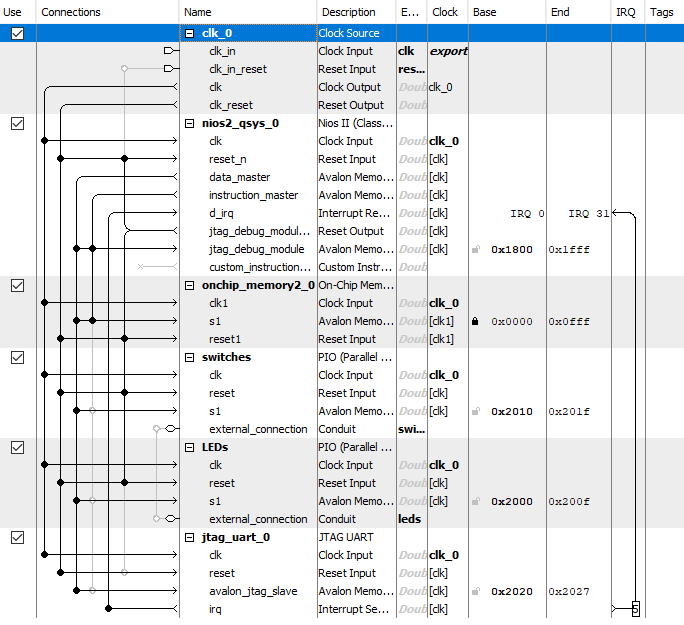
\includegraphics[width=0.9\linewidth]{images/scheme}
		\caption{Проект в $Platform designer$ этап 1}
		\label{fig:scheme}
	\end{figure}
	
	\begin{enumerate}
		\item Для чего нужны регистры, и что будет, если изменить значение регистра r с номером = ваш вариант \% 3 + 2.
		
		Регистры нужны для хранения информации.
		Если изменить значение в 4 регистре, то вскоре программа перезапишет значение в этом регистре на значение, которое пришло изи процессора.
		Если успеть изменить значение в этом регистре сразу после перезаписи процессора, то введенное значение окажется на светодиодной ленте.
		
		\item Что находится в закладке Memory? Модифицируйте значение по адресу 0x00002000 на значение 0x003FFD06. К чему это привело, и почему?
		
		В этой вкладке отображается RAM.
		Из ячейки по адресу 0x00002000 значение передается на светодиодную ленту.
		Модификация значения по адресу 0x00002000 приведет к тому что со следующим тактовым импульсом записанное значение передастся на светодиодную ленту.
	\end{enumerate}

	\subsection{Этап 2}

	Согласно мануалу был создан проект, на рис. \ref{fig:scheme} приведено использование процессора Nios2 в $Platform designer$.
	К процессору подсоединена память и свой модуль вывода информации, а также модуль генерации тактовых импульсов.
	
	Добавление своих компонентов сильно расширяет возможности разработчика.
	Можно создавать свои модули, которых может не быть в библиотеке, а также расширять возможности имеющихся.
	В данном проекте выводится полноценное слово (32 бита) в отличие от предыдущего этапа, где выводилось только 8 битов.
	Также в этот раз уменьшена задержка при отображении результатов.
	
	\begin{figure}[h]
		\centering
		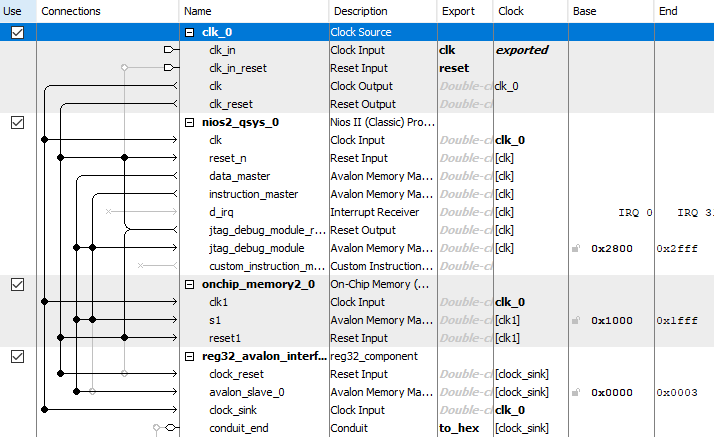
\includegraphics[width=0.9\linewidth]{images/scheme1}
		\caption{Проект в $Platform designer$ этап 2}
		\label{fig:scheme1}
	\end{figure}
	

	\section{Самостоятельная работа}
	
	\subsection{Этап 1}
	
	Далее были подготовлены программ 00\_counter/, 01\_fibonacci/ и 02\_sqrt/ для процессора процессоре Nios II.
	
	00\_counter:
	
	{\small \VerbatimInput{../programs/counter_n.s}}
	
	01\_fibonacci:
	
	{\small \VerbatimInput{../programs/fibonacci_n.s}}
	
	02\_sqrt:
	
	{\small \VerbatimInput{../programs/sqrt_n.s}}
	
	Найти сумму геометрической прогрессии (количество членов прогрессии = 10, знаменатель прогрессии = 8).
	
	Код:
	
	{\small \VerbatimInput{../programs/sum_n.s}}
	
	\subsection{Этап 2}
	
	Программы 00\_counter/, 01\_fibonacci/ и 02\_sqrt/ отличаются от предыдущего этапа тем, что у них не задаются значения через свичи и изменен адрес по-которому записывается результат.
	В остальном программы работают точно также.

	\section{Выводы по работе}
	
	В ходе работы был получен опыт работы в Platform designer.
	Был получен опыт в создании своих компонентов в Platform designer.
	Был изучен порядок работы с памятью и процессором NIOS II.
	Было изучено взаимодействие проекта в с элементами ввода/вывода на плате.
	Был получен опыт в написании кода на ассемблере для процессора NIOS II.
	Был получен опыт в написании кода на языке verilog.
	Итоговый проект был собран и загружен на плату при помощи программы Intel FPGA Monitor Program.

	
	\newpage 
	\renewcommand{\refname}{{\normalsize Список использованных источников}} 
	\centering 
	\begin{thebibliography}{9} 
		\addcontentsline{toc}{section}{\refname} 
		\bibitem{Harris} Хэррис Д. М., Хэррис С. Л. Цифровая схемотехника и архитектура компьютера. – 2015.
	\end{thebibliography}
	
\end{document} % конец документа
